\section{Tracea -- a DSL for traceability}
A DSL\footnote{We use the DSL term to refer to Domain-Specific Modeling Languages, which is the subset of DSLs that are relevant to us} is defined through three main components \cite{kleppe2008-DSLs-with-metamodels}: abstract syntax, concrete syntax, and semantics. 

The abstract syntax defines both the language concepts and their relationships, and also includes well-formedness rules constraining the models that can be created. Metamodeling techniques are normally used to define the abstract syntax. The concrete syntax defines a notation (textual, graphical or hybrid) for the concepts in the abstract syntax, and a translational approach is normally used to provide semantics, though most of the time it is not explicitly formalized.

The metamodel definition directly includes some of the terminology discussed in the previous section. For other concepts we have made sure the DSL is complete enough to allow for that kind of processing or analysis. 
For instance, the concept of traces transcribes directly into classes of the metamodel (\textit{e;g.,} traces, links, artefacts). Processes span over subsets of classes (\textit{e.g.,} granularity and typing).
Characteristics such as vertical traceability, or implicit traces do not appear directly in the metamodel but are either found disseminated among its structural composition or the DSL elements allow for their implementation in specific use cases. 

In this section,
\begin{itemize}
    \item We provide a running example: transclusion for traceability between certification documents and design models.
    \item We present the metamodel, decomposed into five sub-areas of traceability and detail each of them. We reuse the example to show the soundness of our choices.
    \item We provide a textual syntax in the form of a {JSon-based grammar}. 
\end{itemize}

\subsection{Illustrative example: Certification and Design Transclusion }
\begin{figure}[ht]
	\centering 
	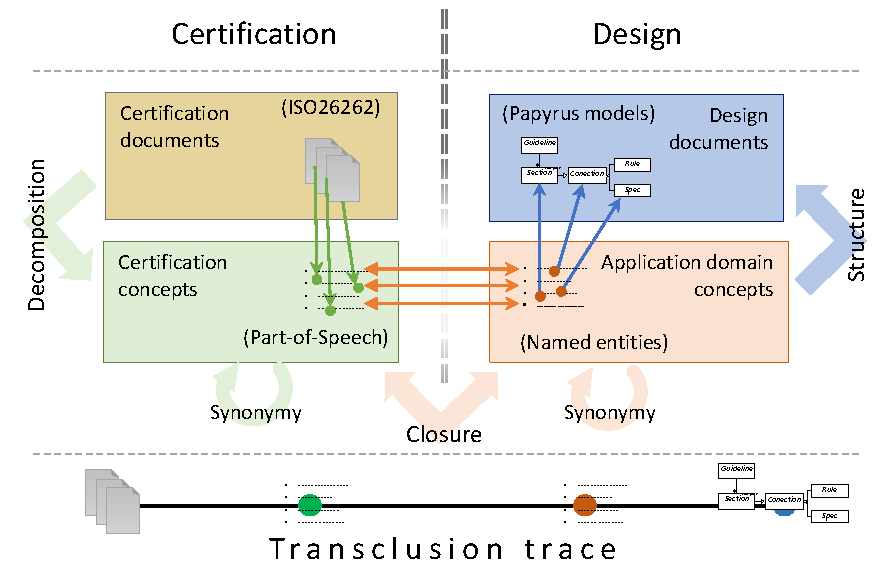
\includegraphics[width=.85\linewidth]{images/metamodel-re}
	\caption{Transclusion of part-of-speech to model entities.}
	\label{fig:metamodel-re}
\end{figure}
 
Certification documents are external to the software system they are certifying. This means that when the software evolves, the content of these documents must be reevaluated to see if the new version of the system can still satisfies the certification conditions. Ideally we would only like to examine the certificate against the changes. And similarly for any change in the certification rules or conditions. We would like that only those parts of the system potentially being affected need to be reviewed and adapted if necessary. 
To be able to support this ``incremental'' evaluations and facilitate the  co-evolution of certification and design artefacts, we need to keep track of the links between the nominal expressions in certifications documents and the elements of design models they target or impact. 
 
As can be seen on the certification side in Figure \ref{fig:metamodel-re}, nominal expressions form semantically rich patterns (\textit{e.g.,} nominal groups, action verbs, nouns, acronyms). They are spread among the sections of the certification documents. The patterns of Parts-of-Speech (PoS) can be extracted using natural language processing  techniques\footnote{The quality of PoSs vary depending on the technique used, its parameterization, as well as the dataset used for training. These choices remain mostly arbitrary and evidences of the superiority of one algorithm or method upon the others remain haphazard~\cite{zou2010-term-based-enhancement-for-trace-retrieval}. In this report, we aim at conceptualizing the problem domain, we do not provide details on the choice and parameterization of such techniques.} 
%\ugh{Maybe ref to annexes with Figure "Linking PLM (decisions) to Papyrus (implementation)" from September CEA meeting.}  

On the design side, named entities are model entities characterized by a unique name (\textit{e.g.,} a method, a class, a package, a model). The structural hierarchy represented by Papyrus models can be used to cluster and disambiguate its constitutive entities~\cite{patel2015-hierarchical-clustering}.
Named entities have synonyms that must be considered as well - and disambiguated when possible.
The association between PoSs and model entities is established with a neural model capable of measuring the (semantic) distance between the elements of both realms\footnote{An interesting methodology to do so is to train a "general intelligence", or to "generally train" a model from available vast corpuses in (more or less) natural language. Then this model is refined with corpuses relevant to the application domain the system belongs to~\cite{shen2015-linking-entities-with-knowledge-base}.}. 
\\
Certification documents are semi-structured text artefacts. Their implementation and validation scenarios may correlate in many different ways with their corresponding modelling entities. We chose the most straight forward case to illustrate an application of the Tracea metamodel: the transclusion of \texttt{PoS} to \texttt{NamedEntities}. Figure \ref{fig:metamodel-re} shows a high level representation of a this process.

This example helps grasp the details of the application of our traceability language to a specific domain: 
%the transclusion of parts of speech in certification documents with their corresponding model elements in Papyrus models. 
an explicit record of the link between important elements of certification and the entities they target in Papyrus models to allow direct transclusion\footnote{A transclusion is the inclusion of part or all of a document into one or more other documents by hypertext reference.}.

Transclusion traces use vertical links (from documents to PoS, and from model to named entity), and horizontal links (between the synonyms and the closure between PoSs and named entities). 
Links related to the composition are explicit: they are contained in the syntax of the domain (\textit{e.g.,} classes are \textit{part} of a package); whereas synonyms and closure are implicit (\textit{i.e.,} they do not appear in the syntax).
This example has a post-requirement nature as it is established after the requirements have been determined.


\subsection{Metamodel} 

\subsubsection{Core structure}\label{sec:core}
\begin{figure}[ht] 
	\centering
	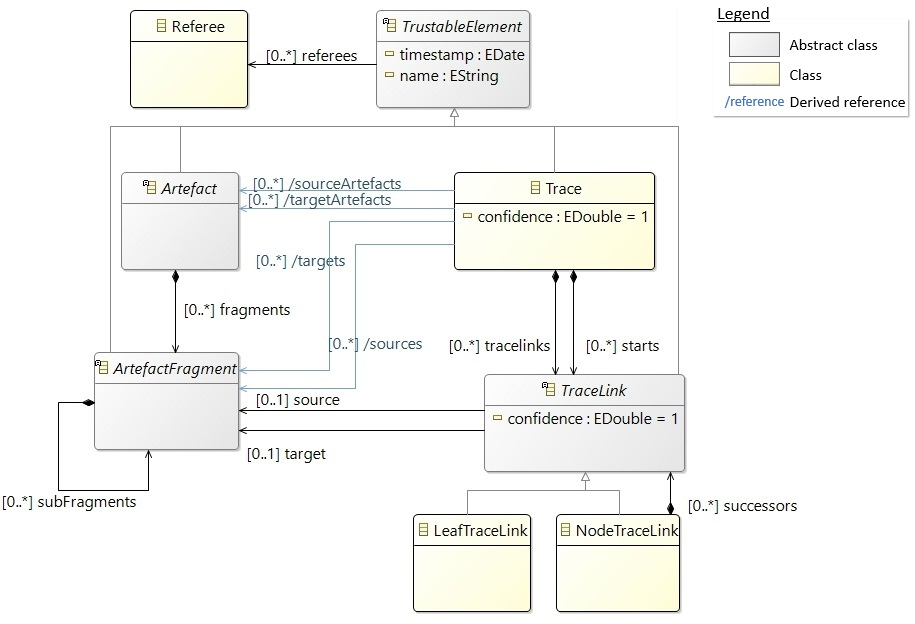
\includegraphics[width=.85\linewidth]{images/core.jpg}
	\caption{Core structure of Tracea metamodel}
	\label{fig:mm-core}
\end{figure}

The core of traceability is to arbitrarily bind artefacts of a system(s) with each others. A trace may have one or many sources and ends with one or many targets. The connection among the artefacts in a trace is expressed as the combination of atomic trace links representing direct connections between a number of fragments of each involved artefact.

Fig. \ref{fig:mm-core} shows an excerpt of Tracea metamodel. This excerpt describes the core structure of traces. It describes the composition scheme of its links (bottom right corner), offers an interface for the decomposition of artefacts into fragments (left side), and allows to record information related to the authorities potentially accountable for its constituents (top class).
%Tracing may refer to \textit{i)} the link between two entities of specific kind: a simple direct link; \textit{ii)} a succession of links from an arbitrary artefact to another; or \textit{iii)} a set of \textit{complex intertwined links}.

\paragraph{Classes}
\begin{itemize}
    \item A \texttt{Trace} is a composition of \texttt{TraceLinks}. It references the source of trace links (\textit{starts} reference) as well as the trace links involved to access the different artefacts (\textit{tracelinks} reference). 
    A trace also references to source and target artefacts and fragments. These references are derived from the \texttt{TraceLinks}.
    \item A \texttt{TraceLink} is the fundamental structure to build the trace sequences and branches. It is a direct connection between two elements of the system (\textit{i.e.,} \texttt{ArtefactFragments}). A \texttt{TraceLink} has one source fragment and one target fragment. It is also the abstract node of a tree of \texttt{TraceLinkNode} and A \texttt{TraceLinkLeaf} refers to a list of successors being part of the linkage of the trace. This class is abstract and is refined into \texttt{NodeTraceLink} and \texttt{LeafTraceLink} following the Composite design pattern.
    \item A \texttt{NodeTraceLink} is a node in a tree like \texttt{TraceLink}. It references successor links.
    \item A \texttt{LeafTraceLink} is a leaf in a tree-like \texttt{TraceLink}. It has no successor link reference.
    \item An \texttt{Artefact} is an abstract representation of an element of the traced system. An artefact represent a text document, a class diagram, or any other kind of document. (See Section~\ref{sec:granularity})
    \item A \texttt{ArtefactFragment} is a part of an Artefact. It can be further decomposed into sub fragments for finer granularity. (See Section~\ref{sec:granularity})
    \item A \texttt{TrustableElement}: Is an abstract class representing elements that have am identifier (name) and a timestamp for timed traceability consideration. It also references \texttt{Referees} to its specializations (\textit{i.e.,} \texttt{Trace}, \texttt{TraceLink}, \texttt{Artefact}, \texttt{ArtefactFragment}, \texttt{Evidence} - see Section \ref{sec:integrity} for details).
    \item A \texttt{Referee} is an actor accountable for a \texttt{TrusteableElement} (See Section~\ref{sec:integrity})
\end{itemize} 

\pagebreak
\paragraph{Well-formedness rules}
Well-formedness rules are expressed as OCL constraints. 
Rules in Figure \ref{fig:ocl-core} ensure that the inclusion of starters in the list of links a trace have, and the derivation of derived references related to source and target artefacts and fragments. 
\begin{figure*}[h]
\centering 
\rule{0.9\linewidth}{1pt}
\vspace{-0.2truecm}
\small
\begin{ocl}[0.85\linewidth]

\vspace{0.3truecm}\OCLcontext~Trace \OCLinv ~starters: \\ \verb+     +\OCLself.tracelinks \OCLarrow includesAll(\OCLself.starts)  

\vspace{0.3truecm}\OCLcontext~Trace \OCLinv ~derivedSources: \\ \verb+     +\OCLself.tracelinks\OCLarrow collect(source) 
\\ \verb+     +\OCLarrow includesAll(\OCLself.sources)   

\vspace{0.3truecm}\OCLcontext~Trace \OCLinv ~derivedTargets: \\ \verb+     +\OCLself.tracelinks \OCLarrow collect(target) 
\\ \verb+     +\OCLarrow includesAll(\OCLself.targets)   

\vspace{0.3truecm}\OCLcontext~Trace \OCLinv ~derivedSourceArtefacts: \\ \verb+     +\OCLself.tracelinks \OCLarrow collect(source)  
\\ \verb+     +\OCLarrow includesAll(\OCLself.sourceArtefacts.fragments)   

\vspace{0.3truecm}\OCLcontext~Trace \OCLinv ~derivedTargetArtefacts: \\ \verb+     +\OCLself.tracelinks \OCLarrow collect(target)  
\\ \verb+     +\OCLarrow includesAll(\OCLself.targetArtefacts.fragments)   

\end{ocl}

\vspace{0.4truecm}
\rule{0.9\linewidth}{1pt}
\vspace{-0.2truecm}

\caption{OCL constraints over elements of the core package.}
\label{fig:ocl-core}
\vspace{-0.6truecm}
\end{figure*}

\paragraph{Illustrative example}
\begin{figure}[h] 
	\centering
	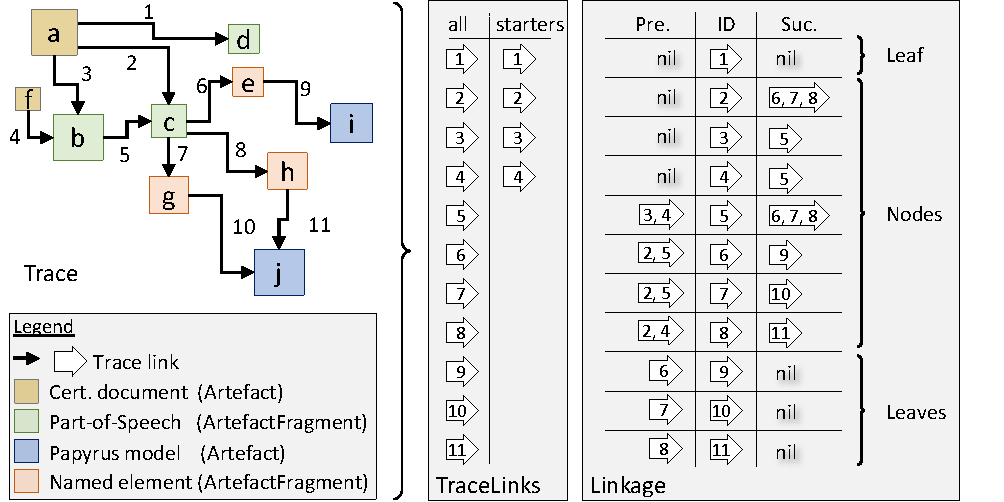
\includegraphics[width=.85\linewidth]{images/core-re}
	\caption{Structure of a transclusion trace. }
	\label{fig:mm-core-instance}
\end{figure}
The core section of the metamodel aims at representing the structure of the linkage between the artefacts that are part of a trace. 
In our example, a trace sequentially links the PoSs in certification documents to their corresponding entities in design models. 
In simple words, a document contains Parts-of-Speech (PoSs) where each PoS is associated to a number of model elements, themselves contained in one or more models. These directions are \texttt{TraceLinks}. Figure \ref{fig:mm-core-instance} shows a diagrammatic perspective of the structure of a transclusion. The example transclusion trace relates the PoS (b, c, and d) of documents (a and f) to the \texttt{NamedElements} (i and j) of three Papyrus models (e, g, h). 
We see on the right side that some \texttt{TraceLinks} have successors, they are \texttt{TraceLinkNode}s; when they do not they are \texttt{TraceLinkLeaf}s. 

When represented as instances of the Tracea metamodel, a certification document is an Artefact, a section of a document is an \texttt{ArtefactFragment}. A PoS is a fragment as well. On the model side, models are \texttt{Artefacts}. Packages, classes, and named elements are \texttt{ArtefactFragments}. We will develop on relationship types in Section \ref{sec:relationshiptype}. 


%Next:  G R A N U L A R I T Y

\subsubsection{Artefact granularity}\label{sec:granularity}

Project stakeholders must decide on the appropriate level of trace granularity for each artifact type. For example, when tracing to UML class diagrams, they could generate a trace at the package, class, or method level.
Granularity must be carefully determined to effectively support stakeholders in their traceability tasks, while minimizing the effort involved to analyze and utilize the set of returned trace links. This can be especially problematic
in large, weakly structured documents that might not contain clearly defined components at the desired granularity level. To mitigate this problem, automated traceability tools can cluster sentences into meaningful semantically related groups and then generate traces to those groups~\cite{clelandhuang2007bestPracticeForAutomatedTraceability}.

As can be seen in Figure \ref{fig:mm-granularity}, We distinguish between five main types of artefacts: i) natural language and unstructured text documents are \texttt{TextArtefacts}, ii) executable test unit and suites are \texttt{TestArtefacts}, iii) models at design or conceptual level are \texttt{ModelArtefacts}, and iv) source code document, SQL sources, scripts and configuration documents are \texttt{CodeArtefacts}. They are all specialization of Artefact. Types differ in the nature of the structure of the artefacts. This is an arbitrary separation grounded on our experience with traceability. Other can be easily introduced to span closer to user needs.
An \texttt{ArtefactFragment} is a part of an Artefact. It can be subdivided into sub-fragments.
\begin{figure}[ht]
	\centering
	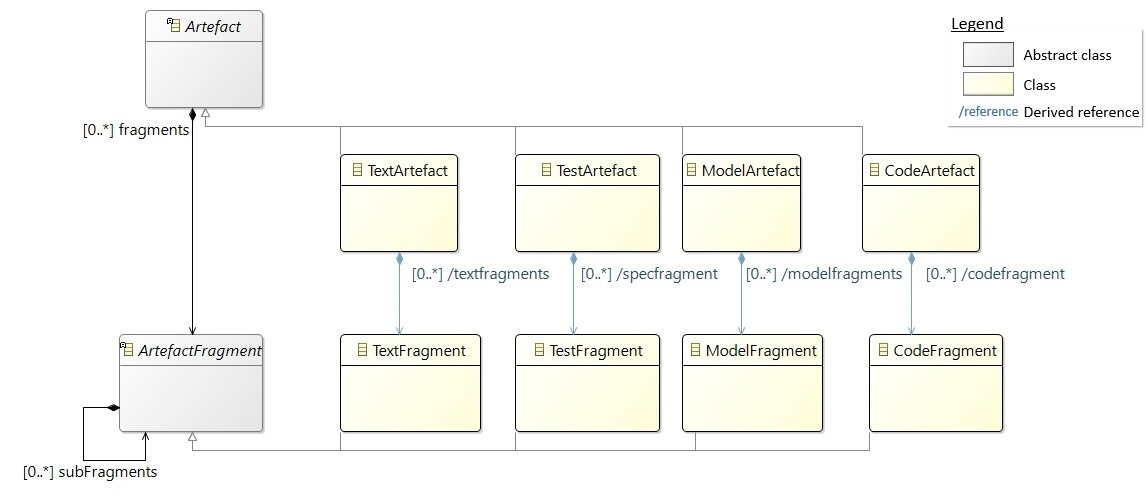
\includegraphics[width=.99\linewidth]{images/granularity.jpg}
	\caption{Customizable granularity}
	\label{fig:mm-granularity}
\end{figure}

Note that we could also opt for a rather simpler approach where artefact types are not modeled as subclasses but where we would just have a single attribute \texttt{ArtefactType} in \texttt{Artefact}. The obvious disadvantage with this option is that we lose the opportunity to add information relevant only to specific types of artefacts.

\paragraph{Classes}
\begin{itemize}
    \item A \texttt{TextArtefact} is a(n) (un)structured text document. \texttt{TextArtefacts} can further decompose into \textit{Sections}, \textit{Subsections}, and \textit{Paragraph}. Each of them may contain \textit{part-Of-Speech} that points to concepts in the application domain.
    
    \item A \texttt{ModelArtefact} is an artefacts related to a model-level representation. \texttt{ModelArtefacts} can be UML, SysML or other types of models, with a structural hierarchy inherent to their entity-relation form. In the case of UML, a decomposition may follow the \textit{Package}, \textit{Class}, \textit{Methods}, \textit{Attributes}, and \textit{References} hierarchical scheme. \textit{Named Elements} point to unique elements of the language uniquely identified.
    
    \item A \texttt{CodeArtefact} is a documents containing source code independently of the specific programming language. \texttt{CodeArtefacts} may decompose into \textit{CodeBlock}, \textit{Header}, \textit{Variable}, \textit{Methods}, and so on. 
    
    \item A \texttt{TestArtefact} is a test unit or suite.
    
    \item And so forth and so on for their respective fragments.
    
\end{itemize}

\pagebreak
\paragraph{Well-formedness rules}
Well-formedness rules are expressed as OCL constraints. 
Rules in Figure \ref{fig:ocl-granularity} the coherence between subtypes of artefacts, fragments, and subfragments. 
\begin{figure*}[h]
\centering 
\rule{0.9\linewidth}{1pt}
\vspace{-0.2truecm}
\small
\begin{ocl}[0.85\linewidth]

\vspace{0.3truecm}\OCLcontext~TextArtefact \OCLinv ~textFragmentsTyping: 
\\ \verb+     + \OCLself.fragments \OCLarrow forAll(\OCLself \OCLarrow oclIsKindOf(TextFragment)

\vspace{0.3truecm}\OCLcontext~CodeArtefact \OCLinv ~codeFragmentsTyping: 
\\ \verb+     + \OCLself.fragments \OCLarrow forAll(\OCLself \OCLarrow oclIsKindOf(CodeFragment)

\vspace{0.3truecm}\OCLcontext~ModelArtefact \OCLinv ~modelFragmentsTyping: 
\\ \verb+     + \OCLself.fragments \OCLarrow forAll(\OCLself \OCLarrow oclIsKindOf(ModelFragment)

\vspace{0.3truecm}\OCLcontext~TestArtefact \OCLinv ~testFragmentsTyping: 
\\ \verb+     +\OCLself.fragments \OCLarrow forAll(\OCLself \OCLarrow oclIsKindOf(TestFragment)


\vspace{0.3truecm}\OCLcontext~TextFragment \OCLinv ~textsubfragmentsTyping: 
\\ \verb+     + \OCLself.subfragments \OCLarrow forAll(\OCLself \OCLarrow oclIsKindOf(TextFragment)

\vspace{0.3truecm}\OCLcontext~CodeFragment \OCLinv ~codesubfragmentsTyping: 
\\ \verb+     + \OCLself.subfragments \OCLarrow forAll(\OCLself \OCLarrow oclIsKindOf(CodeFragment)

\vspace{0.3truecm}\OCLcontext~ModelFragment \OCLinv ~modelsubfragmentsTyping: 
\\ \verb+     + \OCLself.subfragments \OCLarrow forAll(\OCLself \OCLarrow oclIsKindOf(ModelFragment)

\vspace{0.3truecm}\OCLcontext~TestFragment \OCLinv ~testsubfragmentsTyping: 
\\ \verb+     +\OCLself.subfragments \OCLarrow forAll(\OCLself \OCLarrow oclIsKindOf(TestFragment)


\vspace{0.3truecm}\OCLcontext~NamedElement \OCLinv ~noNestedNamedElements: 
\\ \verb+     +\OCLself.namedelementsDefined \OCLarrow isEmpty()  \OCLand
\\ \verb+     +\OCLself.namedelementsUsed \OCLarrow isEmpty() \OCLand
\\ \verb+     +\OCLself.subfragments \OCLarrow isEmpty() 
\end{ocl}

\vspace{0.4truecm}
\rule{0.9\linewidth}{1pt}
\vspace{-0.2truecm}

\caption{OCL constraints over elements of the granularity package.}
\label{fig:ocl-granularity}
\vspace{-0.6truecm}
\end{figure*}


\paragraph{Illustrative example}%Granularity

A trace starts with the PoSs we want to trace down to the design level. It also contains the successive containment connections from document, to section, to PoS in order to refine the granularity of the results to sections instead of whole documents. The trace also contains the link between PoSs and their corresponding model entities, as well as model entities hierarchy (\textit{e.g.,} the class, method, or package they belong to).

To summarize:
\begin{itemize}
    \item A text \texttt{Document} is a \texttt{TextArtefact}. It is decomposed into \texttt{Sections}. Sections define or use \texttt{PoSs}. Both Sections and PoSs are \texttt{TextFragment} (derived from \texttt{ArtefactFragment}).
    \item A Papyrus \texttt{Model} is a \texttt{ModelArtefact}. It is decomposed into modelling elements : \textit{e.g.,} \texttt{Packages}, \texttt{Classes}, and \texttt{Structural features}. They are \texttt{ModelFragments}. \texttt{ModelFragments} (spceializations of \texttt{ArtefactFragments}) define and use \texttt{NamedElements} (\textit{i.e.,} elements of the system with unique identifier). 
\end{itemize}
\begin{figure}[ht]
	\centering
	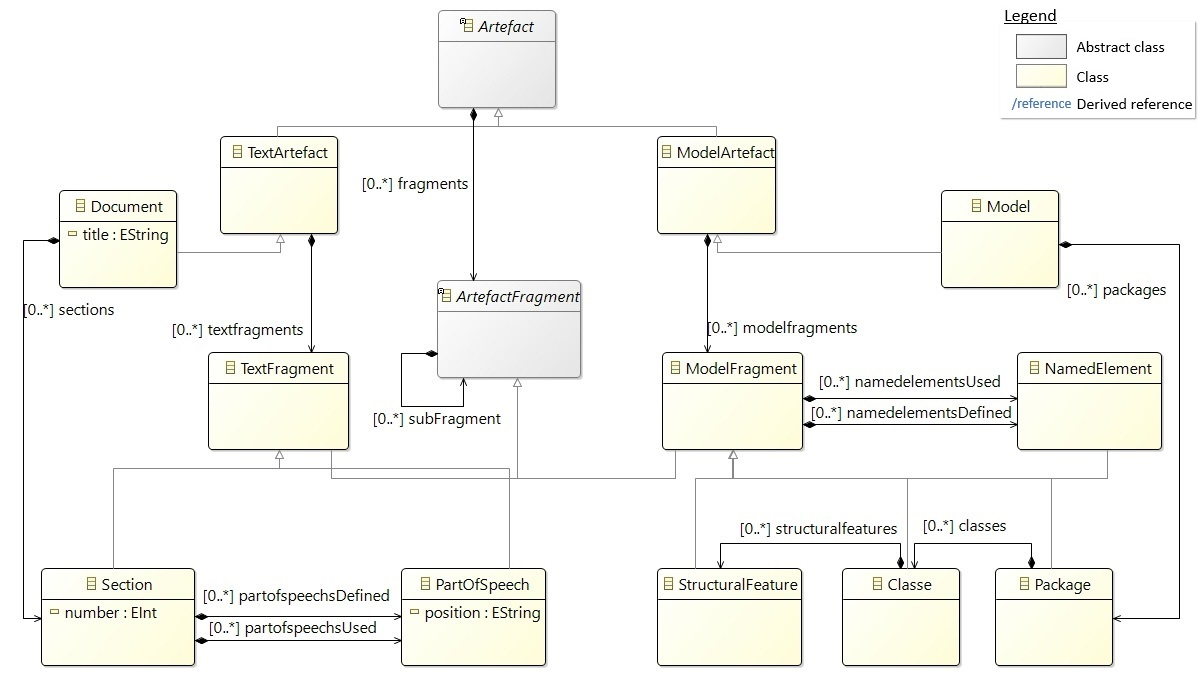
\includegraphics[width=.99\linewidth]{images/granularity-re.jpg}
	\caption{Granularity customized for certification to model transclusion}
	\label{fig:mm-granularity-re}
\end{figure}

\subsubsection{Relationship typing}\label{sec:relationshiptype}

Stakeholders with different perspectives, goals and interests who are involved in software development may contribute to the capture and use of traceability information. Depending on their expertise and needs, they may come up with different types of traceability relations expressing different perspectives on the links among the elements in the project. It is very important to understand project specific conventions for interpreting the meaning of such relations~\cite{Spanoudakis2005} as their semantics will make any traceability analysis much richer and precise.

\begin{figure}[h]
	\centering
	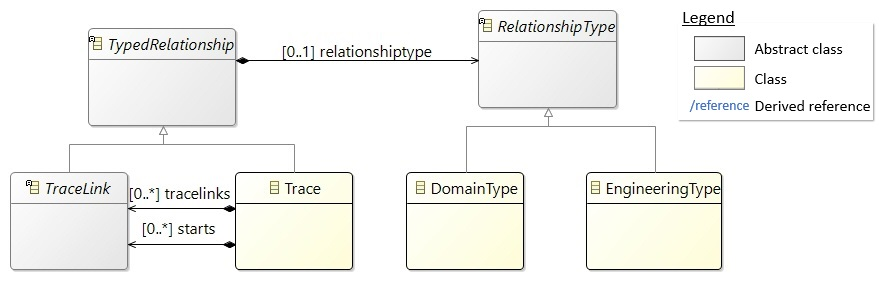
\includegraphics[width=.85\linewidth]{images/relationtyping.jpg}
	\caption{Customizable relationship types}
	\label{fig:mm-relation}
\end{figure}
As can be seen in Figure \ref{fig:mm-relation}, we refine the typing of relationships with a mechanism comparable to UML data typing~\cite{rumbaugh2004-UML2}. A \texttt{TypedRelationship} has an optional \texttt{RelationshipType}. A \texttt{RelationshipType} is abstract and specializes into different levels of sub types.
At the top level, \texttt{DomainType} and \texttt{EngineeringType} define predefined \texttt{RelationshipType}, without any substructure. 

On the one hand we have \texttt{DomainType} types coming from the application domain, used by experts of this domain. They convey semantics of the application domain. On the other hand, \texttt{EngineeringType} are types related to the engineering of software systems and focus on "how" artefacts are related (\textit{i.e.,} implements, Doc2Vec).  We aim to reflect in this architecture the cognitive gap that remains between traceability actors and the users of their product. 

This is an arbitrary separation and other specific types can be easily added to this general design, same as we had for the artefact types. As any metamodel, this one can also be extended to better suit the needs of a specific domain. Some of RelationshipTypes could be generic enough to be reused in different scenarios while others will be very scenario-specific.

\paragraph{Classes}
\begin{itemize}
    \item A \texttt{TypedRelationShip} is an abstract class for the representation of relationships with a type (optional).
    \item A \texttt{RelationshipType} is an abstract class representing a type of relationship.
    \item A \texttt{DomainType} is a \texttt{RelationshipType} dedicated to application domains (\textit{e.g.,} Transclusion).
    \item An \texttt{EngineeringType} is a \texttt{RelationshipType} dedicated to engineering domains (\textit{e.g.,} implements, derives, uses).
\end{itemize}


\paragraph{Constraints}
No constraints.


\paragraph{Illustrative example} %Relationship typing
The types of the links are visible in Figure \ref{fig:mm-relationtyping-re-mm}. They are refinement of \texttt{RelationshipType}. % Six depend on the type of their source and target artefacts (named "\texttt{---2---}"). They are \texttt{EngineeringType} with semantic related to the kind of fragments they reference. 
The three specialized types are \texttt{Transclusion}, \texttt{Closure}, and \texttt{Synonymy}. These are \texttt{DomainType} with semantics related to the reason why two artefacts relate with each other. 
A \texttt{Transclusion} is a complex \texttt{DomainType}. It is a \texttt{Trace} composed of links of different types. We see in Section \ref{sec:integrity} that \texttt{Evidences} are used to record and store parameters and configurations of these more complex kinds of links.

\begin{figure}[ht]
	\centering 
	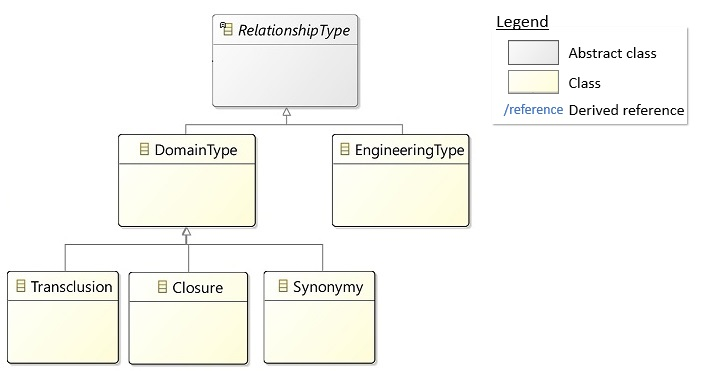
\includegraphics[width=.8\linewidth]{images/relationtyping-re-mm.jpg}
	\caption{Customized relationship typing tailored to transclusion.}
	\label{fig:mm-relationtyping-re-mm}
\end{figure}








\subsubsection{Integrity \& Accountability}\label{sec:integrity}
\begin{figure}[h]
	\centering
	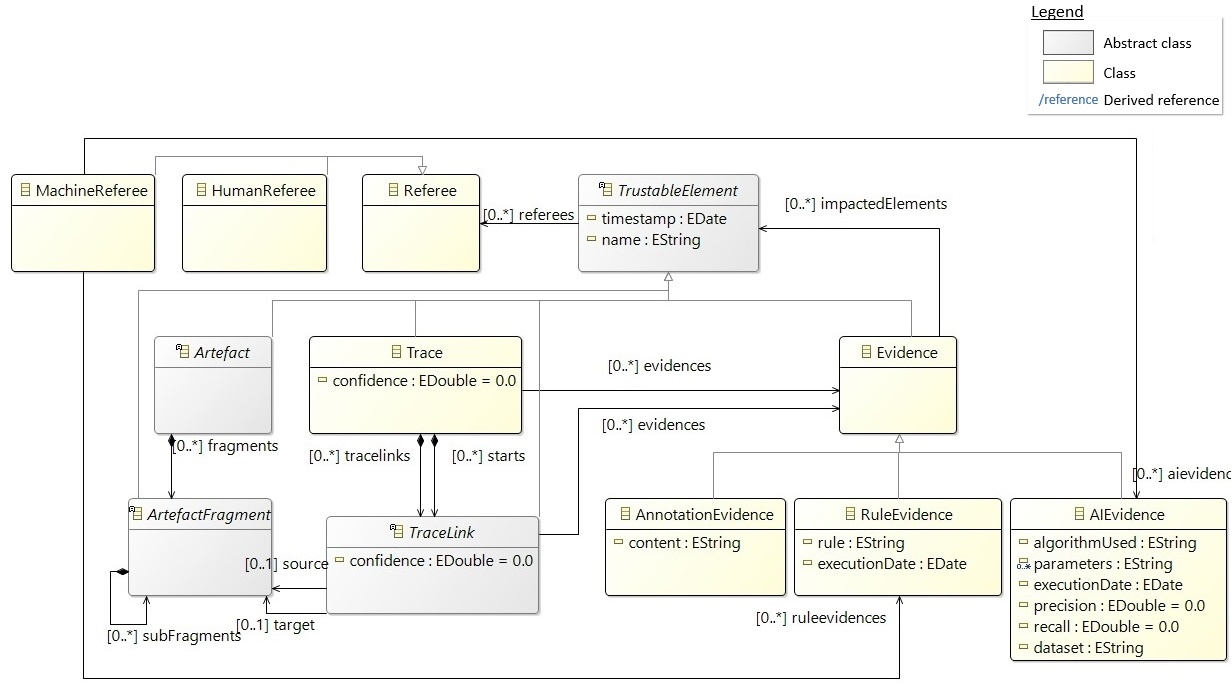
\includegraphics[width=.99\linewidth]{images/integrity.jpg}
	\caption{Integrity}
	\label{fig:mm-integrity}
\end{figure}

When looking at traces is critical to be able to answer questions like "Who is responsible for the creation of this trace?"; "To whom should I refer for more information?"; "How much can I trust this trace is correct?",... If a clear answer is not available, we may lose faith in the whole traceability system or make wrong assumptions on the traceability data that could have very negative impact on the future evolution analysis of the system. 

This is why we believe an explainability mechanism should be a first-class citizen in any traceability approach ~\cite{gotel1995-contribution-structures-req-eng}. Therefore, Tracea brings a dedicated approach to collect, structure, and handle this information.

To begin with, every elements of the Tracea metamodel extends a \texttt{TrusteableElement} (see Figure~\ref{fig:mm-integrity}) as we have seen before. A \texttt{TrusteableElement} contains references to \texttt{Referees} accountable for this element, together with a unique name, and a timestamp.

Beyond this basic support, we also collect evidences for each trace that explain how (and based on what information) that specific trace was created. As such, the \texttt{Evidence} metaclass enables expressing the sets of facts that testify on the means of elicitation, creation, or modification of each elements of a trace. A \texttt{Trace} is potentially linked to a set of evidences. \texttt{Evidence}s are specialized in three subclasses. A trace could be generated as a result of the analysis of a  text annotations with unstructured or grammar-based text explaining the rationale behind such trace (\texttt{AnnotationEvidence}). Or it could be the result of executing a rule (\texttt{RuleEvidence}). Finally, traces can also be the result of the execution of machine learning algorithms and store the type, the ID of the training set, and the precision and recall obtained on that set (\texttt{AIEvidence}).

\texttt{Evidences} increase our certitude that the trace actually exists. Yet, some uncertainty may remind that reflects our belief. We model the (un)certainty a user may have on the quality/existence of the traces with a \textit{confidence} attribute for \texttt{Traces} and \texttt{TraceLinks}. It is a first representation of all the levels of uncertainty that can affect traces (more details in \cite{burgueno2019-uncertainty}).

\paragraph{Classes}
\begin{itemize}
    \item An \textbf{\texttt{Evidence}} is an element that participate in the evaluation of trace reliability. An \texttt{Evidence} references a set of impacted \texttt{TrusteableElements}.
    \item An \texttt{AIEvidence} is an \texttt{Evidence} based on the parameterization and learning precision and recall of an AI algorithm. For example, with traces automatically identified using a machine learning algorithm, an evidence contains the type of the algorithm, its parameters and the level of confidence (\textit{i.e.,} precision and recall on a test bench).
    \item A \texttt{RuleEvidence} is an \texttt{Evidence} describing the execution of integrity rules and their results with a bond to the elements they impact.
    \item An \textbf{\texttt{AnnotationEvidence}}: Textual annotation accounting for Evidence.
    \item A \texttt{Referee} is an actor accountable for a \texttt{TrusteableElement}.
    \item A \texttt{MachineReferee} is a non-human actor responsible for a \texttt{TrusteableElement} (\textit{i.e., } when generated or derived automatically).
    \item A \texttt{HumanReferee}  is a  human actor responsible for a \texttt{TrusteableElement}.
\end{itemize}

\paragraph{Constraints}
No constraints.

\paragraph{Illustrative example}
In our example, \texttt{PoSs} are extracted from certification \texttt{TextDocuments} using natural language processing (NLP) techniques. A \texttt{PoS2NamedEntity} links a \texttt{PoS} and a \texttt{NamedEntity} based on the evaluation of their semantics using machine learning techniques as well. These methods need to be adapted and parameterized, and concrete datasets must be used to train the learning models. We store these attributes in instances of \texttt{AIEvidence} classes. These records will help understand the evolution of the automation.
\begin{figure}[h]
	\centering
	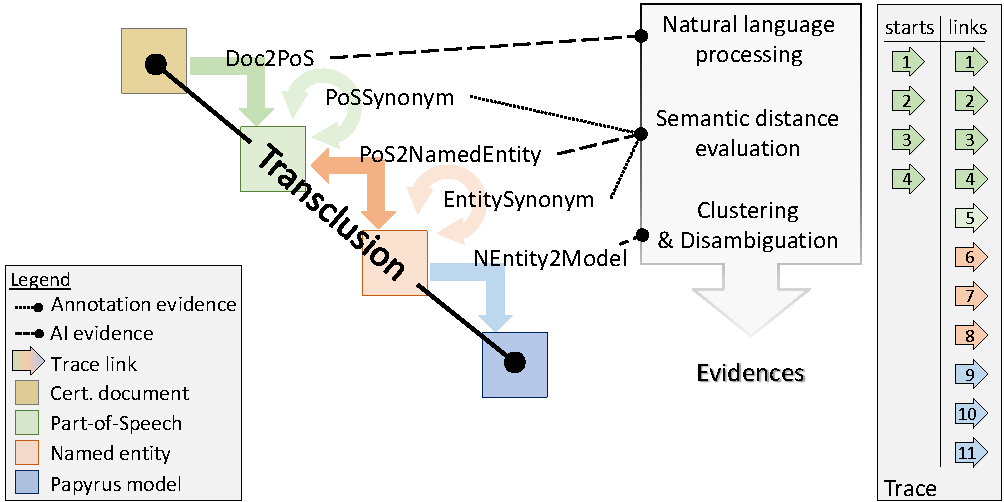
\includegraphics[width=.85\linewidth]{images/relationtyping-re}
	\caption{Complete transclusion process and the record of evidences.}
	\label{fig:mm-relationtyping-re}
\end{figure}
As can be seen in Figure~\ref{fig:mm-relationtyping-re}, we instantiate \texttt{AnnotationEvidence} to record the nature of the synonymy between \texttt{PoSs} and between \texttt{NamedEntities}. 
A \texttt{PoSSynonym} (resp. \texttt{NamedEntitySynonym}) relates two (or more) \texttt{PoS} (reps. \texttt{NamedEntity}) and record the provenance of the evaluation of the distance between the set of elements at play. 

\texttt{Referees} are created for each \texttt{Artifact} and \texttt{Trace} instantiated or modified. The name and the timestamp will provide the useful information to retrieve who is responsible for these elements.



\subsection{Textual Syntax}
\begin{figure}[h]
	\centering 
	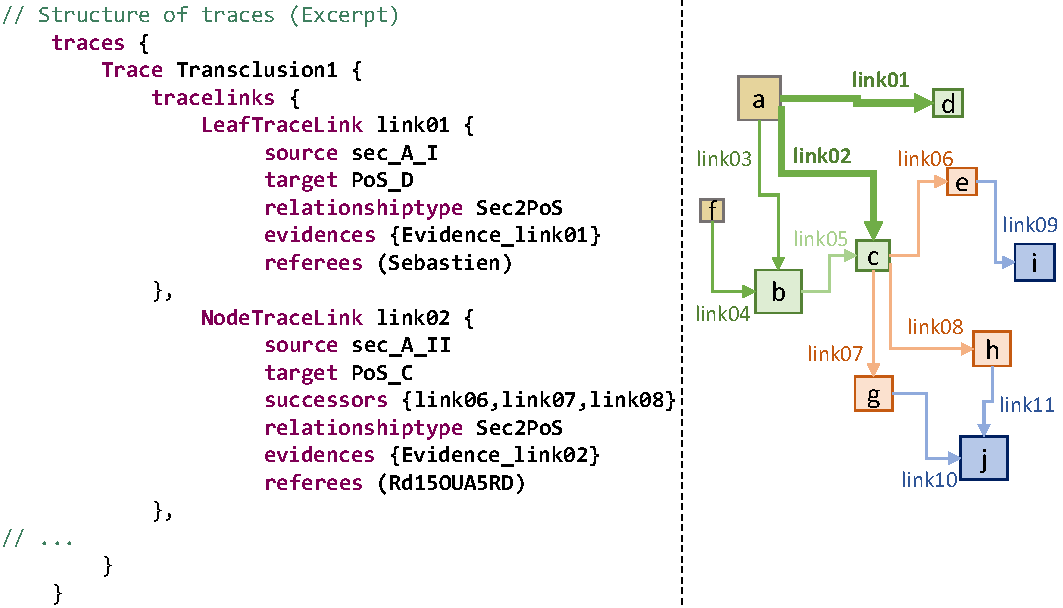
\includegraphics[width=.95\linewidth]{images/listing-struct.pdf}
	\caption{Textual syntax excerpt: core structure of a trace.}
	\label{fig:textualsyntax-struct}
\end{figure}
We chose to use a JSon-like grammar as a first generic textual syntax of Tracea. We believe this type of concrete syntax is appropriate. It is verbose, but \textit{i)} it is readable by humans without holding any structural information from the abstract syntax, and \textit{ii)} known generators can be easily adapted to generate instances. The complete grammar definition has been uploaded on the Modelia Git repository~\cite{Tracea_Repo}.

As can be seen in the excerpt parts of Figure \ref{fig:textualsyntax-struct}, \ref{fig:textualsyntax-declare}, and \ref{fig:textualsyntax-integrity}, classes and structural features of the metamodel are keywords of the grammar. Qualified named are used to navigate into inner elements (\textit{i.e.,} following the pattern \verb|'Root.element.innerElement'| structure with the dot as connector). Elements of a list are set between brackets \verb|{}| and separated with a coma \verb|,|.

\begin{figure}[h]
	\centering 
	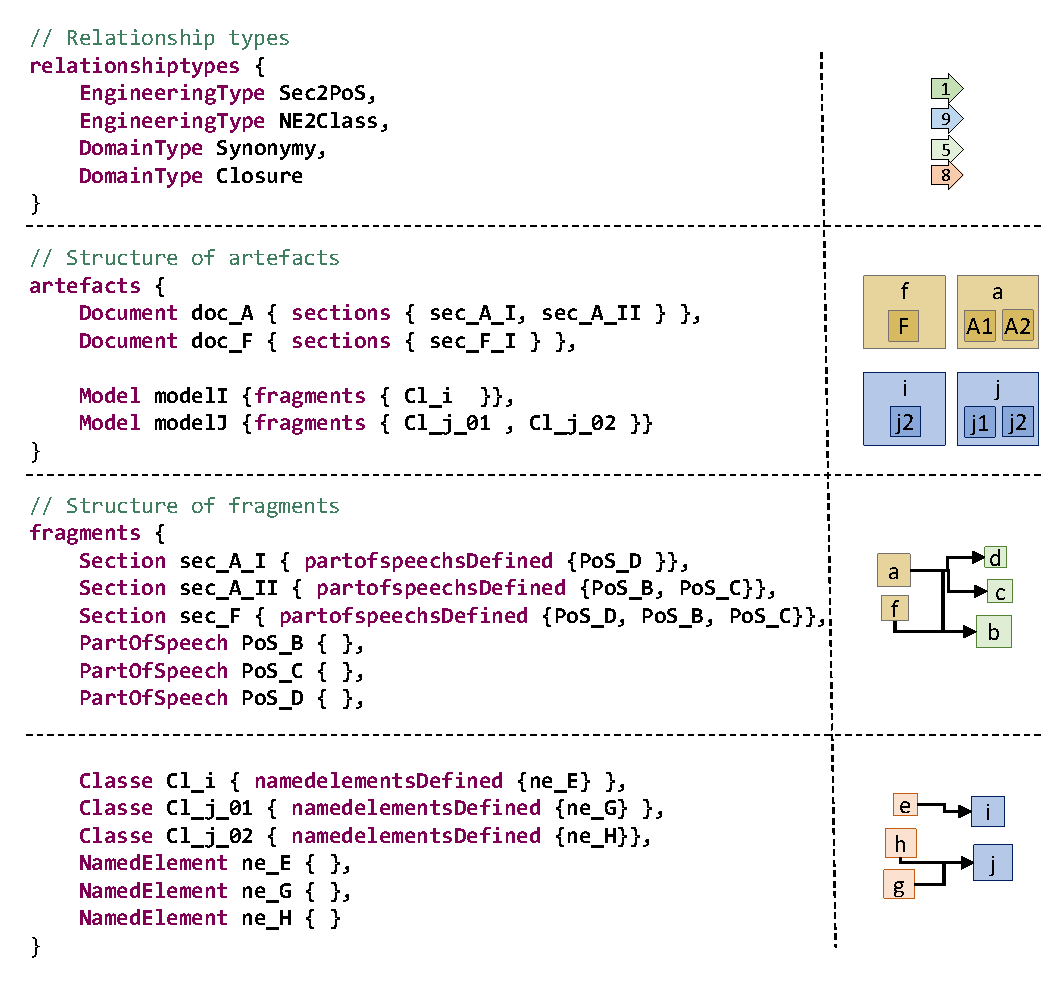
\includegraphics[width=.9\linewidth]{images/listing-art-n-types.pdf}
	\caption{Textual syntax excerpt: artefacts, fragments, and types declarations.}
	\label{fig:textualsyntax-declare}
\end{figure}
In Figure \ref{fig:textualsyntax-struct} \texttt{Traces} are declared sequentially. They contain the declaration of their \texttt{TraceLinks}. Figure \ref{fig:textualsyntax-declare} shows examples of \texttt{RelationshipTypes} declarations, and \texttt{Artefacts} and \texttt{Fragments} decomposition. These elements can be later referenced in different elements of the system. Their dependence level to other elements is weak. In the same manner, Figure \ref{fig:textualsyntax-integrity} presents two \texttt{Evidences} declarations and two \texttt{Referees}.

\begin{figure}[h]
	\centering 
	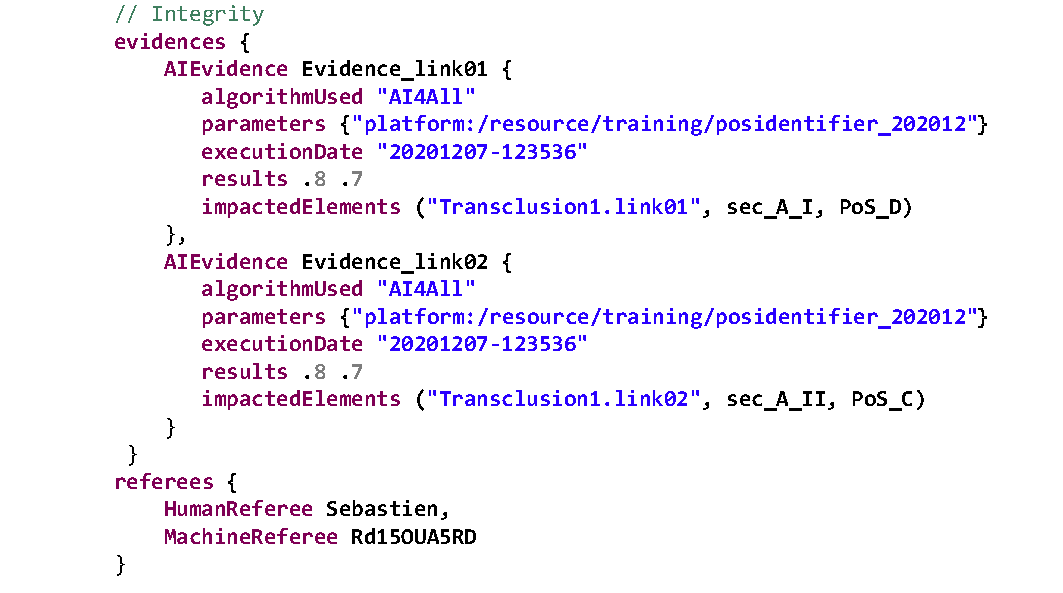
\includegraphics[width=.9\linewidth]{images/listing-integrity.pdf}
	\caption{Textual syntax excerpt: integrity elements declarations.}
	\label{fig:textualsyntax-integrity}
\end{figure}



\subsection{Conclusion and future work}
In this deliverable, we have developed a DSML for traceability. 
In the future, this DSL could be extended with the consideration of belief uncertainty as addressed by Loli Burgueno in the Modelia project~\cite{burgueno2019-uncertainty}. Traceability has an important human factor to consider. This extension would allow reasoning, manipulation and decision making with belief and subjective opinions of the referees involved in the process.

Then, since time plays a fundamental role in the decline of coherence in a system, this dimension shall be investigated meticulously as well. Coordinating the record of tracing operation time wise would give the opportunity to evaluate the aging of traces. In this first version, we simply record \textit{timestamps} for all trusteable artefacts. These stamps shall be augmented with \textit{TemporalEMF}, a profile for temporal metamodelling developed in SOM specifically for EMF solutions~\cite{gomez2018-temporalEMF}.  

Finally, another interesting follow up would be to adapt this DSL to UML, SysML or DOORS in order to populate it with real world traces. This future work requires the evaluation of entry points from Tracea to other languages. It also requires a definition of the purpose of tracing in the projects targeted.

